\chapter*{Введение}\label{Input}
\addcontentsline{toc}{chapter}{Введение}



Параллельные вычисления — способ организации компьютерных вычислений, при котором программы разрабатываются как набор 
взаимодействующих вычислительных процессов, работающих параллельно (одновременно). 

Причины для использования параллелизма:

\begin{enumerate}
  \item разделение обязанностей;
  \item повышение производительности.
\end{enumerate}

Разделение обязанностей почти всегда приветствуется при разработке программ: если сгруппировать взаимосвязанные и разделить 
несвязанные части кода, то программа станет проще для понимания и тестирования и, стало быть, будет содержать меньше ошибок. 

Повысить производительность можно 2 способами: разбить задачу на части и запустить их
параллельно, уменьшив тем самым общее время выполнения и воспользоваться имеющимся параллелизмом для решения
более крупных задач, например, обрабатывать не один файл за раз, а сразу два, десять или двадцать, - способы 
называются распараллеливание по задачам и по данным, соответственно.

Целью данной работы является разработка и исследования параллельных алгоритмов нахождения среднего арифметического матрицы.
Задачами данной лабораторной являются:
\begin{enumerate}
  %\item изучение алгоритмов сортировки пузырьком, вставками, выбором;
  \item реализация последовательного алгоритма нахождения среднего арифметического матрицы;
  \item реализация распараллеленного алгоритма нахождения среднего арифметического матрицы;
  \item сравнительный анализ реализованных алгоритмов;
  \item описание и обоснование полученных результатов в отчете о выполненной лабораторной работе, выполненного как расчетно-пояснительная 
        записка к работе.
\end{enumerate}

\chapter{Аналитическая часть}\label{Analis}
%\addcontentsline{toc}{chapter}{1 Аналитическая часть}

В данном разделе будут рассмотрен алгоритм нахождения среднего арифметического матрицы и
идея его параллельной реализации.

\section{Последовательный алгоритм нахождения среднего арифметического матрицы}\label{BubbleSort}

Последовательно суммируются все элементы матрицы, а после делятся на их количество - строки * столбцы.

\section{Распараллеленный алгоритм нахождения среднего арифметического матрицы}\label{ChoiseSort}

Для увеличения производительности приведенный алгоритм можно распараллелить. Рассмотрим два способа распараллеливания: по строкам и
столбца. В первом случае каждый поток обрабатывает элементы своих строк (эти строки обрабатываются только им). Во втором каждый поток 
обрабатывает элементы своих столбцов.

На рисунке \ref{ris:ill} показан принцип распараллеливания по строкам.

\begin{figure}[H]
  \center{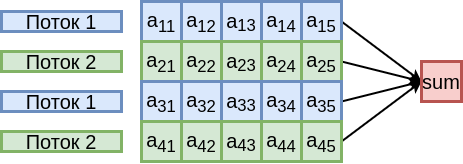
\includegraphics[scale=0.7]{l1.il}}
  \caption{Принцип работы распараллеленого алгоритма}
  \label{ris:ill}
\end{figure}


\section{Вывод аналитической части}\label{End_analis_chapter}

В данной работе стоит задача реализации следующих алгоритмов: последовательного алгоритма нахождения среднего арифметического матрицы,
распараллеленого по строкам алгоритма нахождения среднего арифметического матрицы, распараллеленого по столбцам алгоритма нахождения
среднего арифметического матрицы. Необходимо сравнить алгоритмы умножения матриц по эффективности по времени.
 
